\chapter{Alternativas de desarrollo}\label{alternativas}
La carga de una batería de Li-ion sigue un perfil diseñado para asegurar la seguridad y la vida de estas sin comprometer su rendimiento. Si una batería de Li-ion es descargada completamente, se aplica una precondición de carga de alrededor del 10\%. Esto previene que la pila suba mucho su temperatura hasta un tiempo que sea aceptable enviar 100\% de la corriente hacia la pila como se puede observar en la figura \ref{grafico}.\\
\begin{figure}[H]
\centering
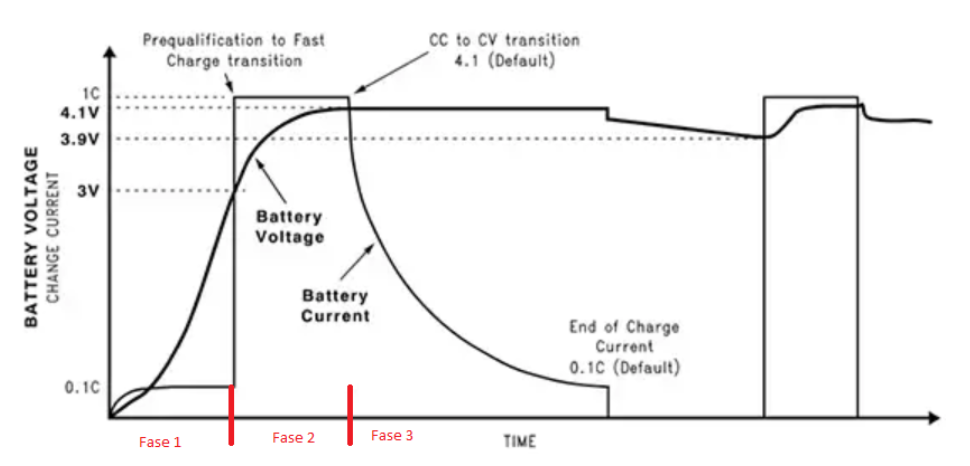
\includegraphics[scale=0.6]{figuras/bateria/grafico.png}
\caption{Etapas de carga de baterías Li-ion para una batería de 4.2[V]}
\label{grafico}
\end{figure}

Como se puede observar en la figura \ref{grafico}, la fase 1 sería la pre-condición de carga del 10\% por un tiempo determinado, luego entra a la fase 2 de corriente al máximo constante y finalmente pasa a la fase 3 donde se mantiene un voltaje constante mientras cae la corriente hasta que termina la carga. 
Cabe destacar que las corrientes se miden en términos de la variable ``C`` la cual se refiere a la corriente que provee la batería, por ejemplo, una batería de $950[mA]$ posee un $C=950$. Esto es importante definir para poder realizar los cálculos de las distintas etapas en el proceso de carga.
\section{Cargador de batería con corriente compartida con carga}
En la actualidad, todos los dispositivos electrónicos tienden a ser lo mas simple posible, es por esto que los diseños que se usan ahora poseen una batería interna que no se puede cambiar o no se deban sacar para cargarlas y así facilitar la tarea al usuario. \\
Esto puede causar un problema debido a la pre-condición que existe en la fase 1 de la figura \ref{grafico}. Si el sistema empieza a pedir mucha corriente implicaría que pueda que no se cumpla esa condición y en ese caso la carga (Arduino) estaría descargando la batería en vez de permitir que se cargue, es por esto que existen integrados que pueden otorgar funcionamiento que permite la interacción de estos.\\
\section{MCP73871}
Considerando un integrado de microchip, el MCP73871\cite{bateria} otorga una funcionalidad de diseñar un sistema que se encargue de cargar una batería de Li-ion con un sistema conectado, que en este caso sería el Arduino. En la tabla \ref{pinesmcp} se muestra la descripción de los pines que se utilizarán en el diseño.\\

\begin{table}[H]
\centering
\begin{tabular}{| c | c | c |}
\hline
\multicolumn{1}{|c|}{\textbf{Nº Pin}}&
\multicolumn{1}{c|}{\textbf{Nombre}}&
\multicolumn{1}{|c|}{\textbf{Función}}\\ \hline
1, 20 & Out & Salida hacia la carga\\ \hline
18, 19 & In & Entrada alimentación\\ \hline
13 & PROG1 & Regulación de corriente de carga rápida\\ \hline
3 & SEL & Selección de input\\ \hline
4 & PROG2 & Límite de corriente entrada USB\\ \hline
12 & PROG3 & Corriente de término de la carga\\ \hline
14, 15 & VBAT & Conexión positiva con la batería\\ \hline
16 & VBAT\_ SENSE & Sensor de voltaje de la batería\\ \hline
\end{tabular}
\caption{Descripción de pines MCP73871}
\label{pinesmcp}
\end{table}

\subsection{Power Supply Input (IN)}
Este viene a ser la conexión a la alimentación en la cual se puede usar un adaptador a la pared USB además de poder cargarlo con un computador. Cuando se usa con la pared se debe considerar que el rango de voltaje debe estar entre $V_{bat} +300[mV]$ y $6[V]$. En este caso no habría problema ya que esta conexión USB provee $5[V]$ y la batería que se va a utilizar es de $3.6 [V]$.

\subsection{Input Source Type Selection (SEL)}
Este pin cumple una función de selección para carga rápida. Con una entrada lógica baja, el limite de carga es de baja corriente $100[mA]$, en cambio al utilizar una entrada lógica alta, la entrada de corriente llega a ser de $500[mA]$. Este pin tiene una relación con la selección del nivel lógico que tenga el pin ''SEL'' como se puede observar en la figura \ref{cargarapida}.\\
\begin{figure}[H]
\centering
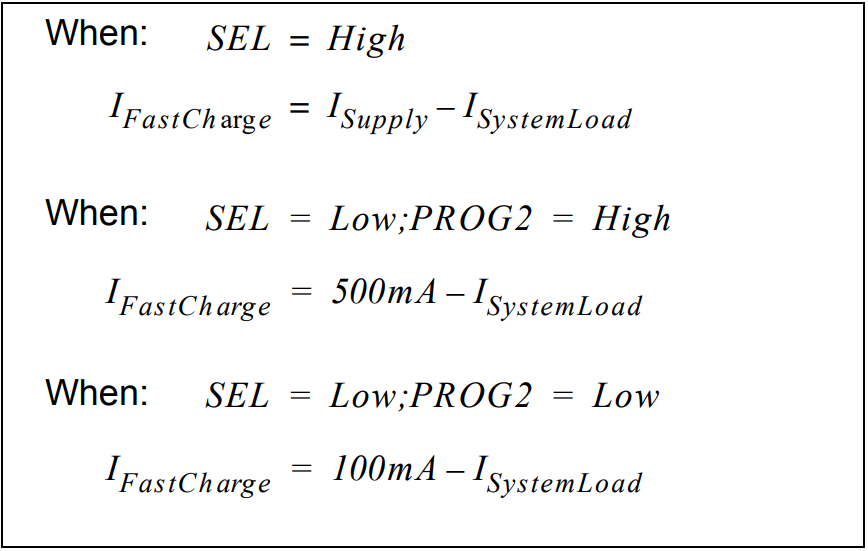
\includegraphics[scale=0.5]{figuras/bateria/cargarapida.png}
\caption{Configuraciones disponibles para carga rápida}
\label{cargarapida}
\end{figure}

Como se puede observar al utilizar ''SEL'' conectado a tierra permite que ''PROG2'' pueda ser utilizado cargando a $500[mA]$ o $100[mA]$ por lo que se elegirá la entrada de ''PROG2'' en alto para que se permita de igual manera cargar rápido y utilizar todas las funciones del dispositivo dejando un límite de seguridad de $500[mA]$.

\subsection{Regulación de carga rápida(PROG1)}
El pin ''PROG1'' determina el máximo constante de corriente con un resistor entre el pin 13 y tierra. Este además fija el máximo de corriente permitida y la corriente de término. Para calcular se debe considerar la ecuación \ref{ivsR}.

\begin{equation}\label{ivsR}
I_{carga} = \frac{1000[V]}{R_{PROG1}[k\Omega]}
\end{equation}

Primero se debe conocer la corriente de carga $I_{Carga}$, para esto se utiliza la ecuación  \ref{calculoRPROG}.
\begin{equation}\label{calculoRPROG}
R_{PROG1} = \frac{1000[V]}{I_{carga}} = 1.315[k\Omega] \approx 1.3[k\Omega]
\end{equation}

Despejando esta ecuación se obtiene un resultado aproximado de $1.3[k\Omega]$ que será la resistencia utilizada para el diseño

\subsection{Corriente de término de carga (PROG3)}

El ciclo de carga es terminado cuando, durante una etapa de voltaje constante (Figura \ref{grafico}), el promedio de corriente disminuye un límite (generalmente 0.1C) que se fija con un resistor conectado desde el pin ''PROG3'' hasta $V_{ss}$ el cual puede ser conectado a tierra.

\begin{equation}\label{Rprog3}
R_{PROG3} = \frac{1000[V]}{I_{Termino}} = 10.5[k\Omega] \approx 10[k\Omega]
\end{equation}

\subsection{Salida de voltaje a la batería $V_{BAT}$ y sensor de voltaje de batería $V_{SENSE}$}

Al conectar el terminal positivo de la batería de Li-ion el pin  $V_{BAT}$ cumple la función de cargarla, es recomendable utilizar un capacitor de cerámico en la salida para que asegure la estabilidad de la carga. 
El pin $V_{SENSE}$ se encarga de entregar el voltaje de salida para que el integrado se pueda realimentar con el valor que está entregando y corregirlo. 

\subsection{Pines Generales}

Los pines mencionados anteriormente son los más relevantes con respecto a diseño del dispositivo, hay otros pines que recomienda el fabricante utilizar como referencia para el usuario o el desarrollador los cuales muestran, conectando diodos led, Estado de batería, estado de carga y si se está entregando o no alimentación al dispositivo. 
Además hay otras funciones que no se utilizan por lo que esos pines son conectados a tierra o al voltaje de alimentación según se especifique.

\subsection{Diseño del esquemático}

Con todos los cálculos anteriores, finalmente se diseña el circuito con el integrado en el programa EagleCAD que será usado para enviar a producción de la PCB como se muestra en la figura \ref{esquematico22}.

\begin{figure}[H]
\centering
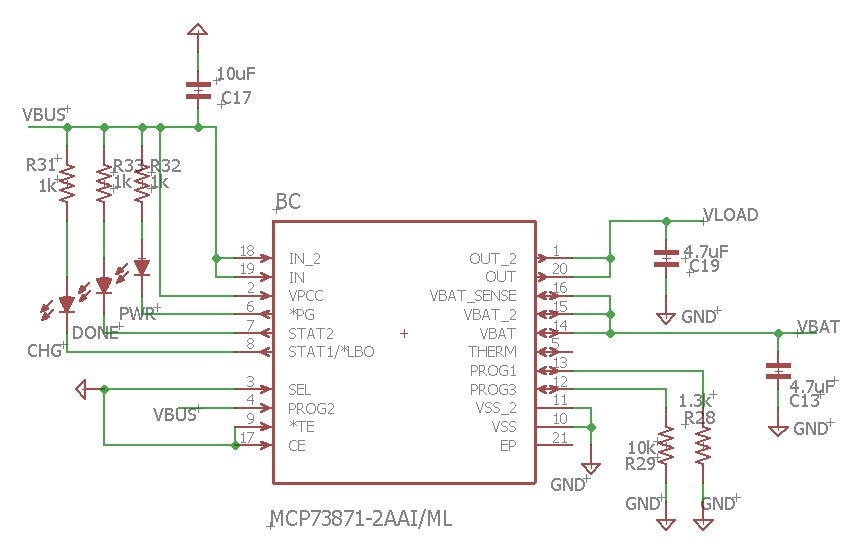
\includegraphics[scale=0.7]{figuras/bateria/esquematico.jpg}
\caption{Diseño de cargador de batería en software EagleCAD}
\label{esquematico22}
\end{figure}

Se puede observar los valores diseñados para una batería de $3.7[V]$ de Li-ion con $950[mAh]$ de capacidad. Como se recomendó en $V_{BAT}$ es necesario utilizar condensadores de cerámica para regular las salidas, al igual que en $V_{LOAD}$ el cual viene a ser el que se entrega al Arduino.\\
Se eligen los valores de ''SEL'' en $0[V]$ y ''PROG2'' en $5[V]$ para así limitar la corriente de carga a la diferencia entre $500[mA]$ y la corriente de la carga, tal como se indica en la figura \ref{cargarapida}.